

\documentclass{beamer}

\mode<presentation> {

% The Beamer class comes with a number of default slide themes
% which change the colors and layouts of slides. Below this is a list
% of all the themes, uncomment each in turn to see what they look like.

%\usetheme{default}
%\usetheme{AnnArbor}
%\usetheme{Antibes}
%\usetheme{Bergen}
%\usetheme{Berkeley}
%\usetheme{Berlin}
%\usetheme{Boadilla}
%\usetheme{CambridgeUS}
%\usetheme{Copenhagen}
%\usetheme{Darmstadt}
%\usetheme{Dresden}
%\usetheme{Frankfurt}
%\usetheme{Goettingen}
%\usetheme{Hannover}
%\usetheme{Ilmenau}
%\usetheme{JuanLesPins}
%\usetheme{Luebeck}
%\usetheme{Madrid}
%\usetheme{Malmoe}
%\usetheme{Marburg}
%\usetheme{Montpellier}
%\usetheme{PaloAlto}
%\usetheme{Pittsburgh}
%\usetheme{Rochester}
%\usetheme{Singapore}
%\usetheme{Szeged}
%\usetheme{Warsaw}

% As well as themes, the Beamer class has a number of color themes
% for any slide theme. Uncomment each of these in turn to see how it
% changes the colors of your current slide theme.

%\usecolortheme{albatross}
%\usecolortheme{beaver}
%\usecolortheme{beetle}
%\usecolortheme{crane}
%\usecolortheme{dolphin}
%\usecolortheme{dove}
%\usecolortheme{fly}
%\usecolortheme{lily}
%\usecolortheme{orchid}
%\usecolortheme{rose}
%\usecolortheme{seagull}
%\usecolortheme{seahorse}
%\usecolortheme{whale}
\usecolortheme{wolverine}

%\setbeamertemplate{footline} % To remove the footer line in all slides uncomment this line
%\setbeamertemplate{footline}[page number] % To replace the footer line in all slides with a simple slide count uncomment this line

%\setbeamertemplate{navigation symbols}{} % To remove the navigation symbols from the bottom of all slides uncomment this line
}

\usepackage{graphicx} % Allows including images
\usepackage{booktabs} % Allows the use of \toprule, \midrule and \bottomrule in tables


\usepackage{listings}
\lstset{language=Java,
                basicstyle=\footnotesize\ttfamily,
                keywordstyle=\footnotesize\color{blue}\ttfamily,
}

%----------------------------------------------------------------------------------------
%	TITLE PAGE
%----------------------------------------------------------------------------------------

\title[OOP]{9.OOP Introduction} % The short title appears at the bottom of every slide, the full title is only on the title page

\author{Sakib Abrar} % Your name
\institute[BUET] % Your institution as it will appear on the bottom of every slide, may be shorthand to save space
{
CSE\\~\\Bangladesh University of Engineering \& Technology \\ % Your institution for the title page
\medskip
\textit{sakib.cghs@gmail.com} % Your email address
}
\date{\today} % Date, can be changed to a custom date

\begin{document}

\begin{frame}
\titlepage % Print the title page as the first slide
\end{frame}

\begin{frame}
\frametitle{Overview} % Table of contents slide, comment this block out to remove it
\tableofcontents % Throughout your presentation, if you choose to use \section{} and \subsection{} commands, these will automatically be printed on this slide as an overview of your presentation
\end{frame}

%----------------------------------------------------------------------------------------
%	PRESENTATION SLIDES
%----------------------------------------------------------------------------------------

%------------------------------------------------
\section{OOP Principles}
%------------------------------------------------

\begin{frame}
\frametitle{OOP Principles}
\begin{itemize}
\item \textbf{Abstraction:} Abstraction means using simple things to represent complexity. We all know how to turn the TV on, but we don’t need to know how it works in order to enjoy it. 
\item \textbf{Encapsulation:} This is the practice of keeping fields within a class private, then providing access to them via public methods. It’s a protective barrier that keeps the data and code safe within the class itself. 
\item \textbf{Inheritance:} This is a special feature of Object Oriented Programming in Java. It lets programmers create new classes that share some of the attributes of existing classes. This lets us build on previous work without reinventing the wheel.
\item \textbf{Polymorphism:} This Java OOP concept lets programmers use the same word to mean different things in different contexts. One form of polymorphism in Java is \textbf{method overloading}. The other form is \textbf{method overriding}. 
\end{itemize}
\end{frame}


%------------------------------------------------

%------------------------------------------------
\section{Java Class}
%------------------------------------------------

\begin{frame}
\frametitle{Java Class}
A class is a template definition of the methods and variables in a particular kind of object.\\~\\
This is a blueprint for some objects that we will create later.\\~\\
In stead of coding it whole everytime, we create a blueprint than reuse it whenerver we need to create an instance.
\end{frame}

%------------------------------------------------
\section{Java Object}
%------------------------------------------------

\begin{frame}
\frametitle{Java Object}
An object is an instance of the class. Class is like a variable type and object is the variable. \\~\\
Class is the template where we put our data the objects get created.
\end{frame}

%------------------------------------------------
\section{Class Object Example}
%------------------------------------------------


\begin{frame}[fragile]{Example}
\begin{columns}[T]
% code
\begin{column}{\textwidth}
\begin{lstlisting}
class Car {
    int wheels = 4;
    int price = 100;
    String model = "Toyota";
}

public class OOPExamples {
    public static void main(String[] args) {
        Car amarGari = new Car();
        System.out.println(amarGari.model);
    }
}
\end{lstlisting}
\end{column}
% description
\end{columns}
\end{frame}



%-----------------------------------------------
\section{Java Constructors}
%-----------------------------------------------

\begin{frame}{Java Constructors}
\textbf{You don't always want your car model to be toyota.}\\
You may want to be able to change your objects attributes while creation.\\That was the whole point of the OOP. The template must be capable of creating different attribuited objects on the go.\\And here comes the constructors to the rescue.\\~\\
\textbf{A constructor in Java is a special method that is used to initialize objects. The constructor is called when an object of a class is created. It can be used to set initial values for object attributes.}
\end{frame}


%-----------------------------------------------
\section{Constructor Examples}
%------------------------------------------------

\begin{frame}[fragile]
\frametitle{Constructor Examples}
\begin{columns}[T]
% code
\begin{column}{\textwidth}
\begin{lstlisting}
class Car {
    int wheels;
    int price;
    String model;

    public Car(int wheels, int price, String model) {
        this.wheels = wheels;
        this.price = price;
        this.model = model;
    }
}

\end{lstlisting}
\end{column}
% description
\end{columns}
\end{frame}

%------------------------------------------------


%------------------------------------------------

\begin{frame}[fragile]
\frametitle{Constructor Examples}
\textbf{You can also overload constructors:}
\begin{columns}[T]
% code
\begin{column}{\textwidth}
\begin{lstlisting}
class Car {
    int wheels;
    int price;
    String model;

    public Car(int wheels, int price, String model) {
        this.wheels = wheels;
        this.price = price;
        this.model = model;
    }

    public Car(int price, String model) {
        this.wheels = 4;
        this.price = price;
        this.model = model;
    }
}

\end{lstlisting}
\end{column}
% description
\end{columns}
\end{frame}

%------------------------------------------------


%-----------------------------------------------
\section{Default Constructor}
%------------------------------------------------

\begin{frame}
\frametitle{Default Constructor}
If you don’t implement any constructor in your class, the Java compiler inserts default constructor into your code on your behalf. \\You will not see the default constructor in your source code(the .java file) as it is inserted during compilation and present in the bytecode(.class file).\\~\\
The default constructor is inserted by compiler and has no code in it, on the other hand we can implement no-arg constructor in our class which looks like default constructor but we can provide any initialization code in it.
\end{frame}

%------------------------------------------------



%------------------------------------------------
\section{Access Modifiers in Java}
%------------------------------------------------

\begin{frame}
\frametitle{Access Modifiers}
\begin{itemize}
\item \textbf{Private:} The access level of a private modifier is only within the class. It cannot be accessed from outside the class.
\item \textbf{Default:} The access level of a default modifier is only within the package. It cannot be accessed from outside the package. If you do not specify any access level, it will be the default.
\item \textbf{Protected:} The access level of a protected modifier is within the package and outside the package through child class. If you do not make the child class, it cannot be accessed from outside the package.
\item \textbf{Public:} The access level of a public modifier is everywhere. It can be accessed from within the class, outside the class, within the package and outside the package.
\end{itemize}
\end{frame}


%------------------------------------------------

\begin{frame}
\frametitle{Understanding Java Access Modifiers}
\textbf{Let's understand the access modifiers in Java by a simple table:}\\~\\
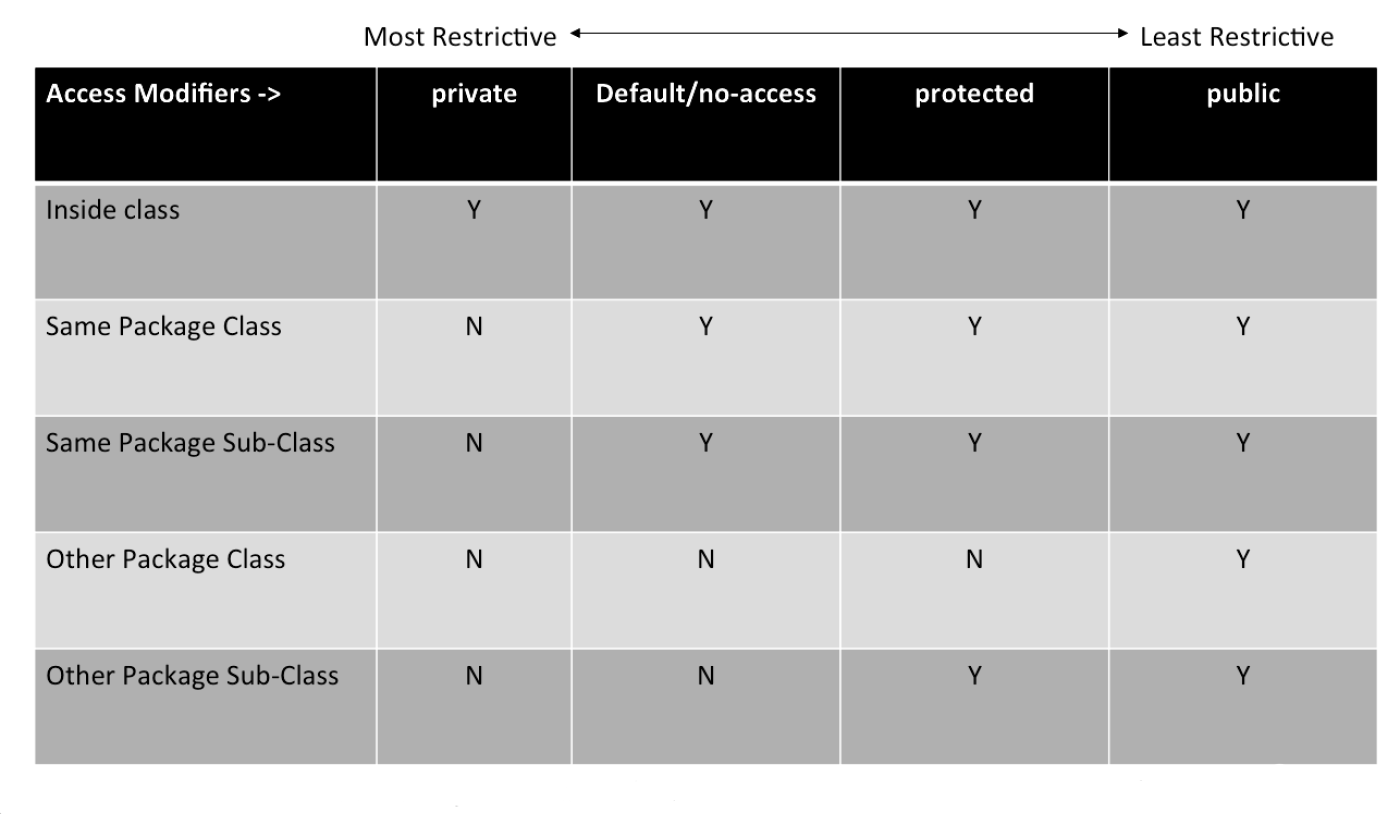
\includegraphics[width=\textwidth]{AccessModifier.png}
\end{frame}

%--------------------------------------------------

\begin{frame}
\Huge{\centerline{THE END }}
\end{frame}

%----------------------------------------------------------------------------------------

\end{document} 